\subsection{Bounding the Optimum}

\begin{defn}[Approximation Algorithm]
	An algorithm \texttt{A} is an \textbf{$\alpha$-approximation} ($\alpha \geq 1$) for a problem $Q$ if for every instance $I$,
	\begin{enumerate}
		\item \texttt{A} outputs a feasible solution \texttt{S}
		\item \texttt{A} runs in polynomial time
		\item If $Q$ is a minimization problem, then cost$(\texttt{S}) \leq \alpha \cdot $ cost$(\texttt{OPT})$
		\item If $Q$ is a maximization problem, then val$(\texttt{S}) \geq 1/\alpha \cdot $ val$(\texttt{OPT})$
	\end{enumerate}
\end{defn}

\subsection{Application 1: Travelling Salesman Problem}
Suppose that we are given a complete, undirected graph $K_n$ with non-negative integer costs $c$ for each edge. The goal is to find the cheapest Hamiltonian cycle of $G$.

\begin{defn}[Triangle Inequality]
	The edge-cost function $c: V(K_n) \times V(K_n) \rightarrow \mathbb{R}^+$ satisfies the \textbf{triangle inequality} if the following holds,
	\[c\underbrace{(v_1, v_2)}_{e_1} \leq c\underbrace{(v_1, v_3)}_{e_2} - c\underbrace{(v_3, v_2)}_{e_3} \quad \forall e_1, e_2, e_3 \in E(K_n)\]
\end{defn}

\begin{marginfigure}
	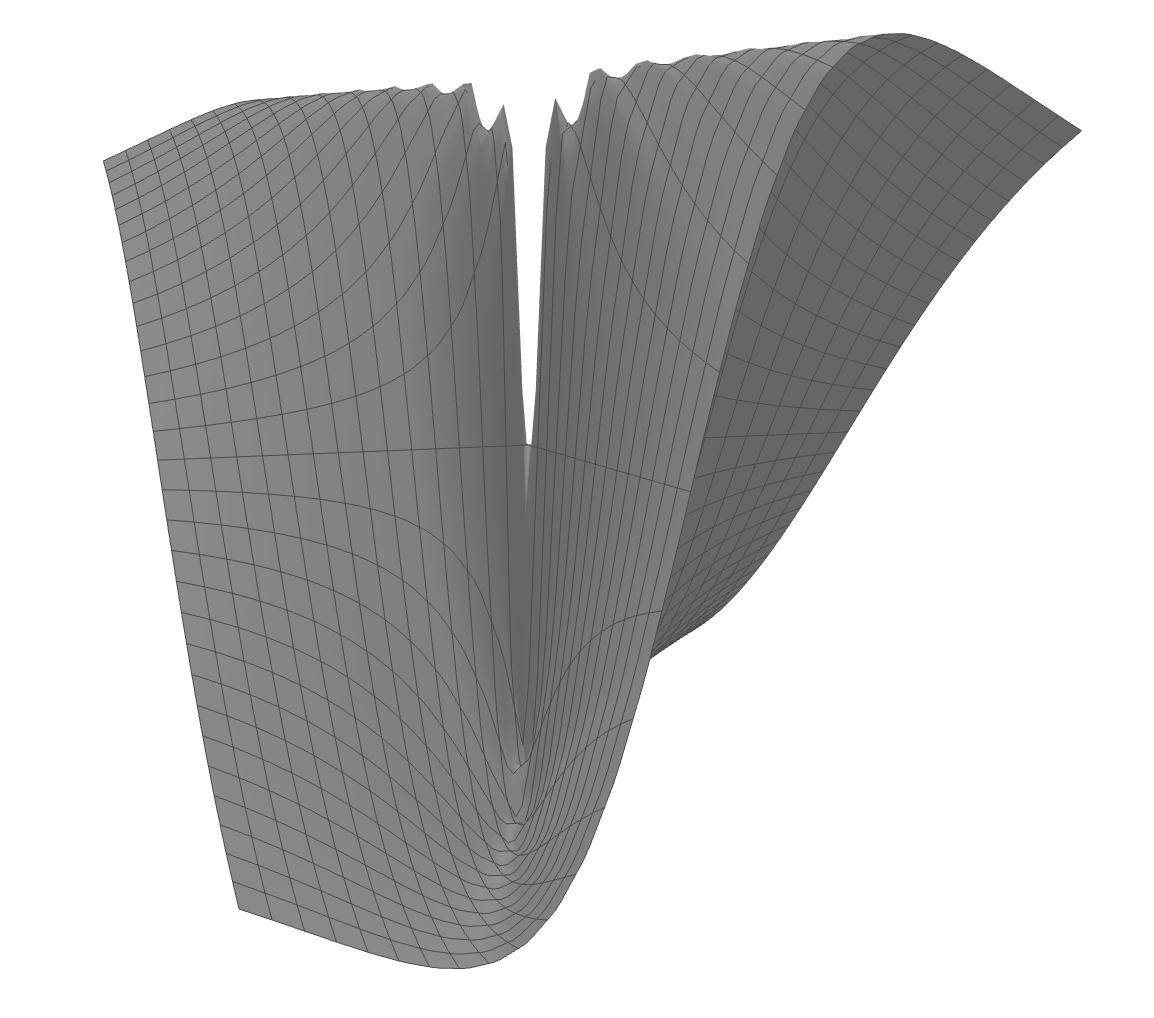
\includegraphics[width=\textwidth]{fig-22.png}
	\caption{Illustration of metric costs.}
\end{marginfigure}

\begin{defn}[Walk]
	A \textbf{walk} is a sequence of vertices,
	\[v_1, \cdots, v_n \text{ such that } (v_i, v_j) \in E(G) \text{ for all $i,j \in [n]$}\]
\end{defn}

\begin{defn}[Eulerian Graph]
	Let $G = (V, E)$ be a multigraph. $G$ is \textbf{Eulerian} if it has a closed walk that uses every edge exactly once.
\end{defn}

\begin{marginfigure}
	\begin{enumerate}
		\item A \textbf{path} is a walk with no vertex repeated, while a \textbf{trail} is a walk with no edge repeated.
		\item An \textbf{Euler trail} is a trail that uses every edge, and an \textbf{Euler tour} is a closed Euler trail.
	\end{enumerate}
\end{marginfigure}

\begin{thm}[2-Approximation TSP]
	The \texttt{TreeDoubling} algorithm is a \textbf{2-approximation algorithm} for the Metric TSP.
	\begin{algorithm}
	  \caption{2-Approximation Travelling Salesman}\label{2approxTSP}
	  \Comment{$\texttt{Prim}(G, c)$ uses Prim's Algorithm to find a minimum spanning tree in $G$, given the weight function $c$}
	  \Function{TreeDoubling($K_n$, $c$)}{
	  	\Comment{Find a minimum spanning tree $T$ of $K_n$}
	  	$T \assign \FuncCall{Prim}{$K_n$, $c$}$\;
	  	\Comment{Duplicate each edge in $T$ to obtain a Eulerian multigraph $T^{\prime}$ (all vertex degrees in $T^{\prime}$ are even)}
	  	$T^{\prime} \assign (V(K_n) \text{, } 2 \cdot E(T))$\;
		\Comment{Compute a Eulerian tour $H$ of $T^{\prime}$. Whenever a vertex $v$ is visited in $H$ that was already visited, skip $v$ and proceed with the next unvisited node along the cycle}
	  	$H \assign \FuncCall{PreOrder}{$T^*$}$\;
	  	\Comment{Return resulting Hamiltonian tour $H$}
	  	\Return{$H$}\;
	  }
	\end{algorithm}
\end{thm}

\begin{proof}
 	\texttt{TreeDoubling} is a 2-approximation algorithm if,
	\begin{enumerate}
		\item It outputs a feasible tour $H$
		\item It runs in polynomial time
		\item Its cost is at most $2 \cdot c(\texttt{OPT})$
	\end{enumerate}

	\noindent Polynomial running time is guaranteed since \texttt{Prim} runs in $O(|V(K_n)|^2)$ and \texttt{PreOrder} is a form of Depth First Search, which is in $O(|V(K_n)| + |E(K_n)|)$. Moreover, the \texttt{TreeDoubling} algorithm clearly outputs a feasible solution since $H$ is a Eulerian tour by construction.

	It remains to prove that $c(H) \leq 2 \cdot \texttt{OPT}$, where \texttt{OPT} is the optimal tour in $K_n$. Let $T$ be a minimum spanning tree of $K_n$ with respect to $c$. We know that $c(T) \leq c(\texttt{OPT})$ since deleting any edge of a Hamiltonian tour gives a spanning tree. Therefore,
	\begin{align*}
		c(H) &\leq c(2 \cdot T) \text{ by short-cutting} \\
			 &= 2 \cdot c(T) \\
			 &\leq 2 \cdot (\texttt{OPT})
	\end{align*}
	\noindent Thus, we have an approximation algorithm with $\alpha = 2$.
\end{proof}

\begin{marginfigure}
	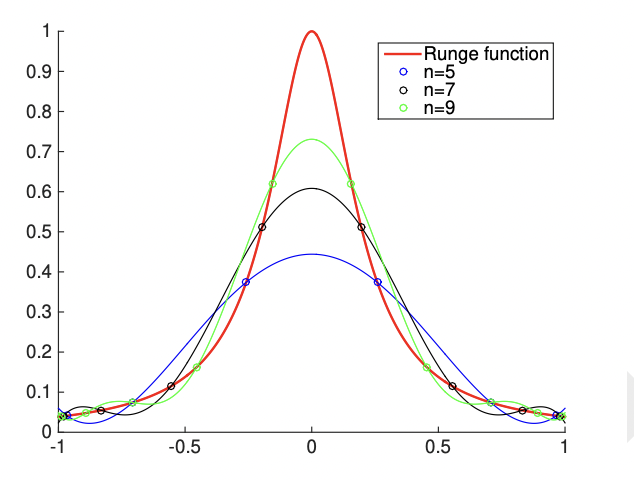
\includegraphics[width=\textwidth]{fig-23.png}
	\caption{Illustration of the \texttt{TreeDoubling} algorithm.}
\end{marginfigure}

\begin{marginfigure}
	Suppose that  $H^{\prime}$ is a lower bound for \texttt{OPT}. We can ask \textbf{four questions},
	\begin{enumerate}
		\item Is the analysis tight with respect to the lower bound for \texttt{OPT}? Find an example where $c(H) = \alpha \cdot H^{\prime}$
		\item Is the lower bound for \texttt{OPT} closer to \texttt{OPT} than a factor of 2? Find an example where $\texttt{OPT} = \alpha \cdot  H^{\prime}$
		\item Is the analysis tight with respect to \texttt{OPT}? Find an example where $c(H) = \alpha \cdot \texttt{OPT}$
		\item Is there a better approximation algorithm for our problem?
	\end{enumerate}
\end{marginfigure}

The natural question that arises is whether an approximation guarantee of $\alpha = 2$ is sufficient. There are four questions to ask,
\begin{enumerate}
	\item Is our analysis tight with respect to the lower bound $T$? Yes.
	\begin{center}
			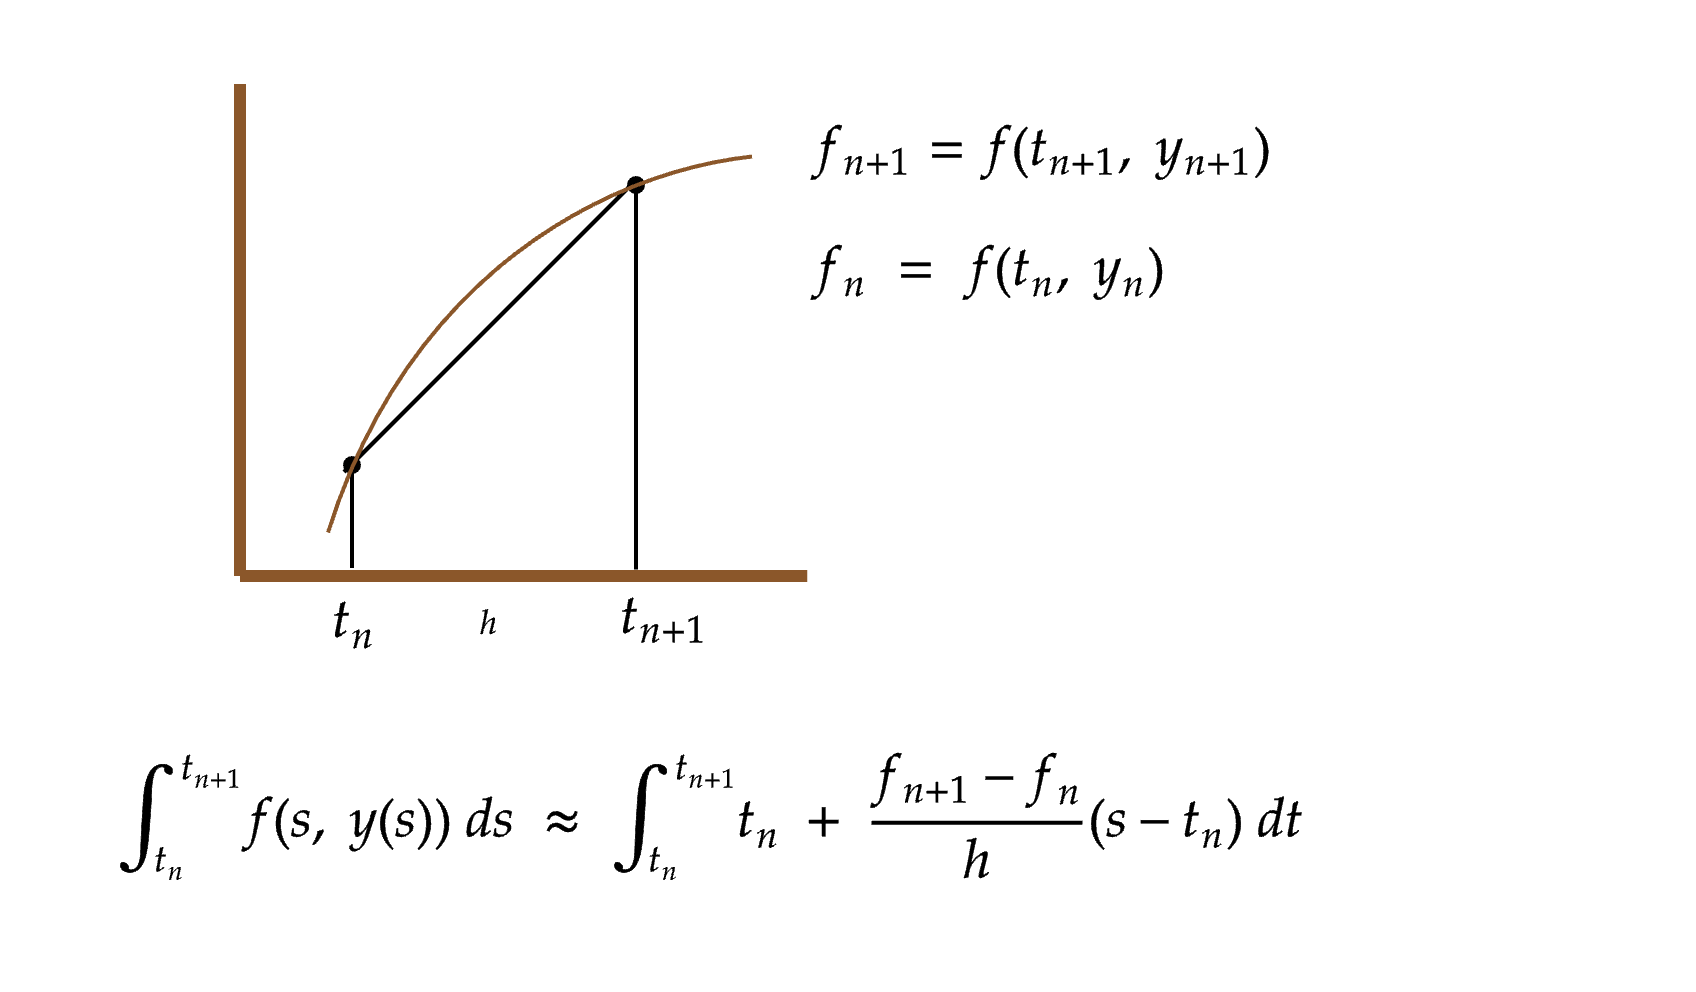
\includegraphics[width=\textwidth]{fig-24.png}
	\end{center}

	\item Is the lower bound closer to \texttt{OPT} than a factor of 2? No.
	\begin{center}
			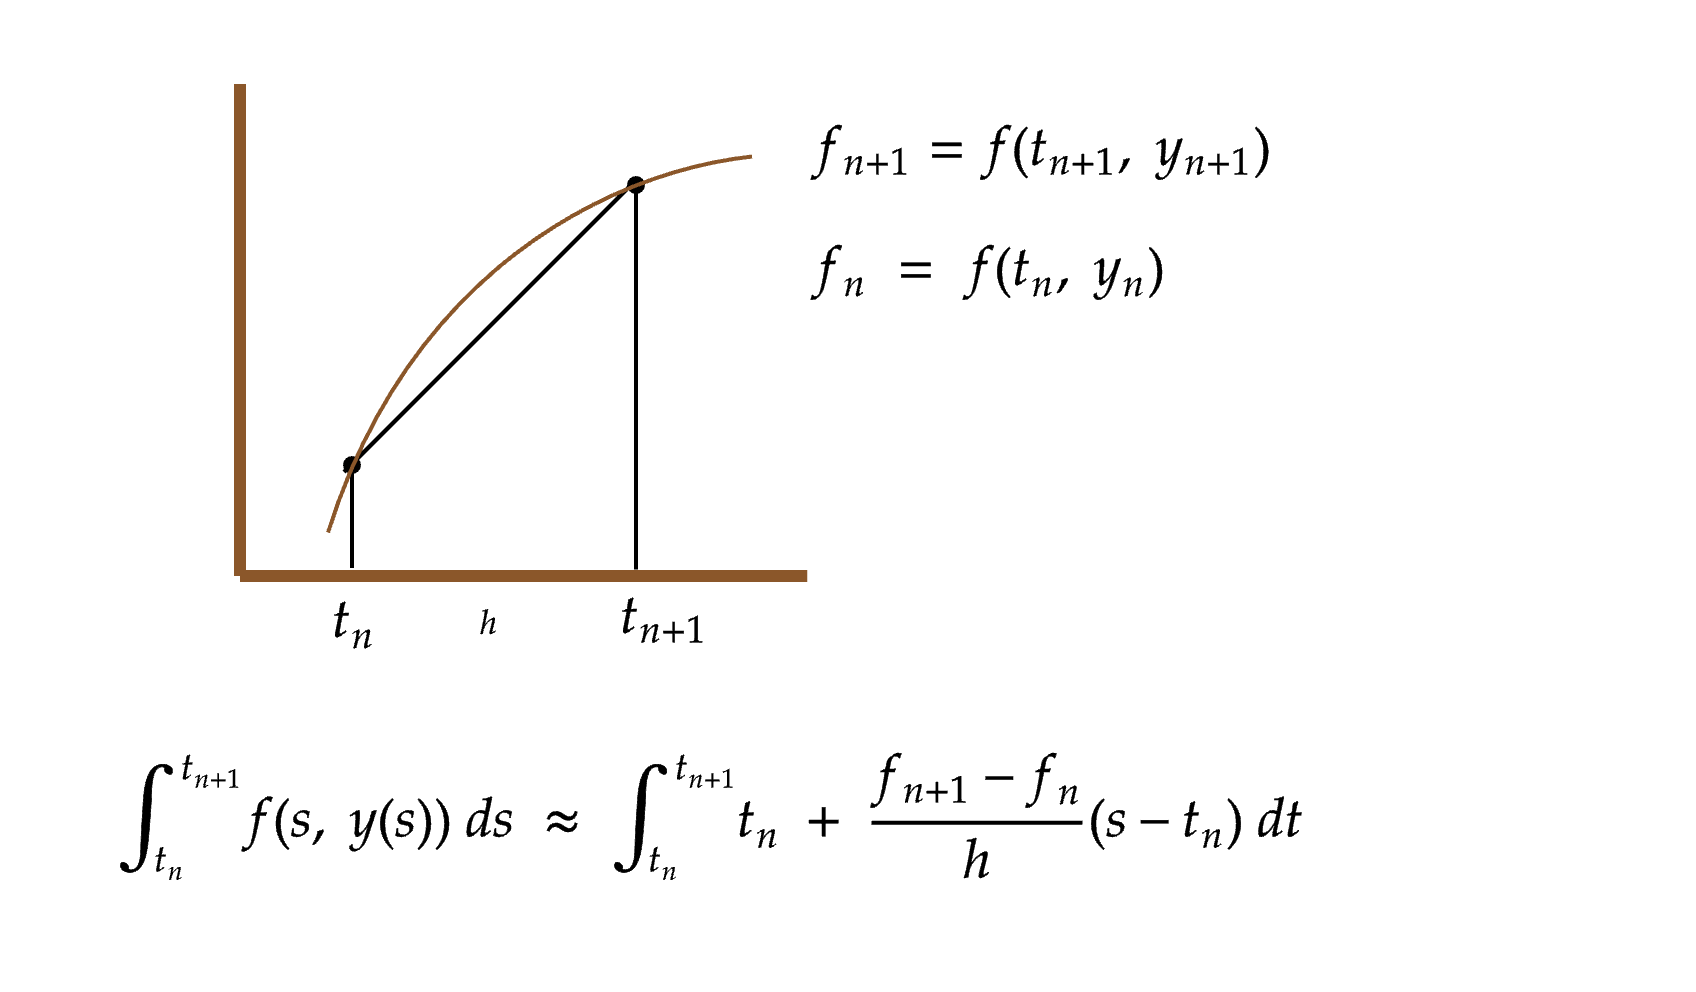
\includegraphics[width=\textwidth]{fig-24.png}
	\end{center}

	\item Is the analysis tight with respect to \texttt{OPT}? Yes.
	\begin{center}
			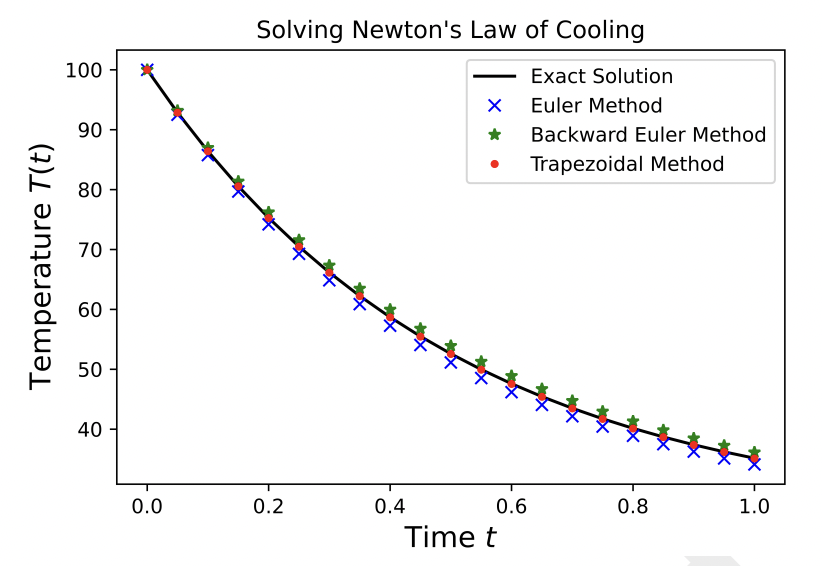
\includegraphics[width=\textwidth]{fig-25.png}
	\end{center}

	\item Is there a better approximation algorithm?
	\noindent Yes. there is a $\frac{3}{2}$-approximation algorithm for the metric TSP.
\end{enumerate}

\begin{marginfigure}
	See the following \href{https://link.springer.com/content/pdf/10.1007%2F978-0-387-30162-4_230.pdf}{paper} for more information on the Metric TSP.

\end{marginfigure}

\begin{defn}[Matching on a Set]
	A matching $M$ of $G$ is called a \textbf{matching on $U \subseteq V(G)$} if all edges of $M$ consist of two vertices from $U$\footnote{Recall that the matching is called "perfect" if every vertex of $U$ is incident with an edge of $M$.}. 
\end{defn}

\begin{thm}[3/2-Approximation TSP]
	The \texttt{Christofides} algorithm is a \textbf{3/2-approximation algorithm} for the Metric TSP\footnote{Instead of doubling the number of edges, we can add edges between odd degree vertices. The graph will still have even degree vertices and therefore an Euler tour.}.
	\begin{algorithm}
	  \caption{3/2-Approximation Travelling Salesman}\label{23approxTSP}
	  \Comment{$\texttt{Prim}(G, c)$ uses Prim's Algorithm to find a minimum spanning tree in $G$, given the weight function $c$}
	  \Function{Christofides($K_n$, $c$)}{
	  	\Comment{Find a minimum spanning tree $T$ of $K_n$}
	  	$T \assign \FuncCall{Prim}{$K_n$, $c$}$\;
	  	\Comment{Let $U \subseteq V(T)$ be the odd degree vertices in $T$}
	  	$U \assign \{v \mid v \in V(T) \text{ and deg}(v) = 2k+1\}$\;
	  	\Comment{Compute a minimum weight perfect matching $M$ on the subgraph induced by $U$}
	  	$M \assign \FuncCall{Ford-Fulkerson}{$K_n$, $U$, $c$}$\;
	  	\Comment{Compute a Eulerian tour $H$ of $T \cup M$, taking shortcuts to obtain a Hamiltonian tour}
	  	$H \assign \FuncCall{PreOrder}{$T^*$}$\;
		\Return{$H$}\;
	  }
	\end{algorithm}
\end{thm}

\begin{proof}
	\texttt{Christofides} is a 3/2-approximation algorithm if,
	\begin{enumerate}
		\item It outputs a feasible tour $H$
		\item It runs in polynomial time
		\item Its cost is at most $3/2 \cdot c(\texttt{OPT})$
	\end{enumerate}

	\noindent First observe that the number of odd degree vertices of the spanning tree $T$ is even, since the sum of the degrees of all vertices is $2(n-1)$ by the Handshaking Lemma. Thus, a perfect matching on $U$ exists. Moreover, it can be found using maximum flows in $O(n^3)$. Hence, the algorithm is polynomial. Moreover, the \texttt{Christofides} algorithm outputs a feasible solution since $H$ is a Eulerian tour by construction.

	The weight of the Eulerian tour $H$ is at most $c(T) + c(M)$, and it was proven earlier that $c(T) \leq \texttt{OPT}$\footnote{$c(H) < c(T) + c(M)$ by shortcutting and applying the triangle inequality.}. It suffices to show that $c(M) \leq \frac{1}{2} \cdot \texttt{OPT}$, where \texttt{OPT} is the optimal tour in $K_n$.

	Since \texttt{OPT} is a Hamiltonian Cycle, we can shortcut to obtain a cycle $\hat{C}$ on the set of odd degree vertices. Clearly $|\hat{C}| = |U|$, so $\hat{C}$ can be partitioned into two matchings $M_1, M_2$. In particular,
	\begin{align*}
		\frac{1}{2}\left(\texttt{OPT} \right) &= \frac{1}{2}\left(c(M_1) + c(M_2)\right) \\
											  &\geq c(M)
	\end{align*}
	\noindent since $M$ was computed to be the minimum weight perfect matching.
\end{proof}

\begin{marginfigure}
	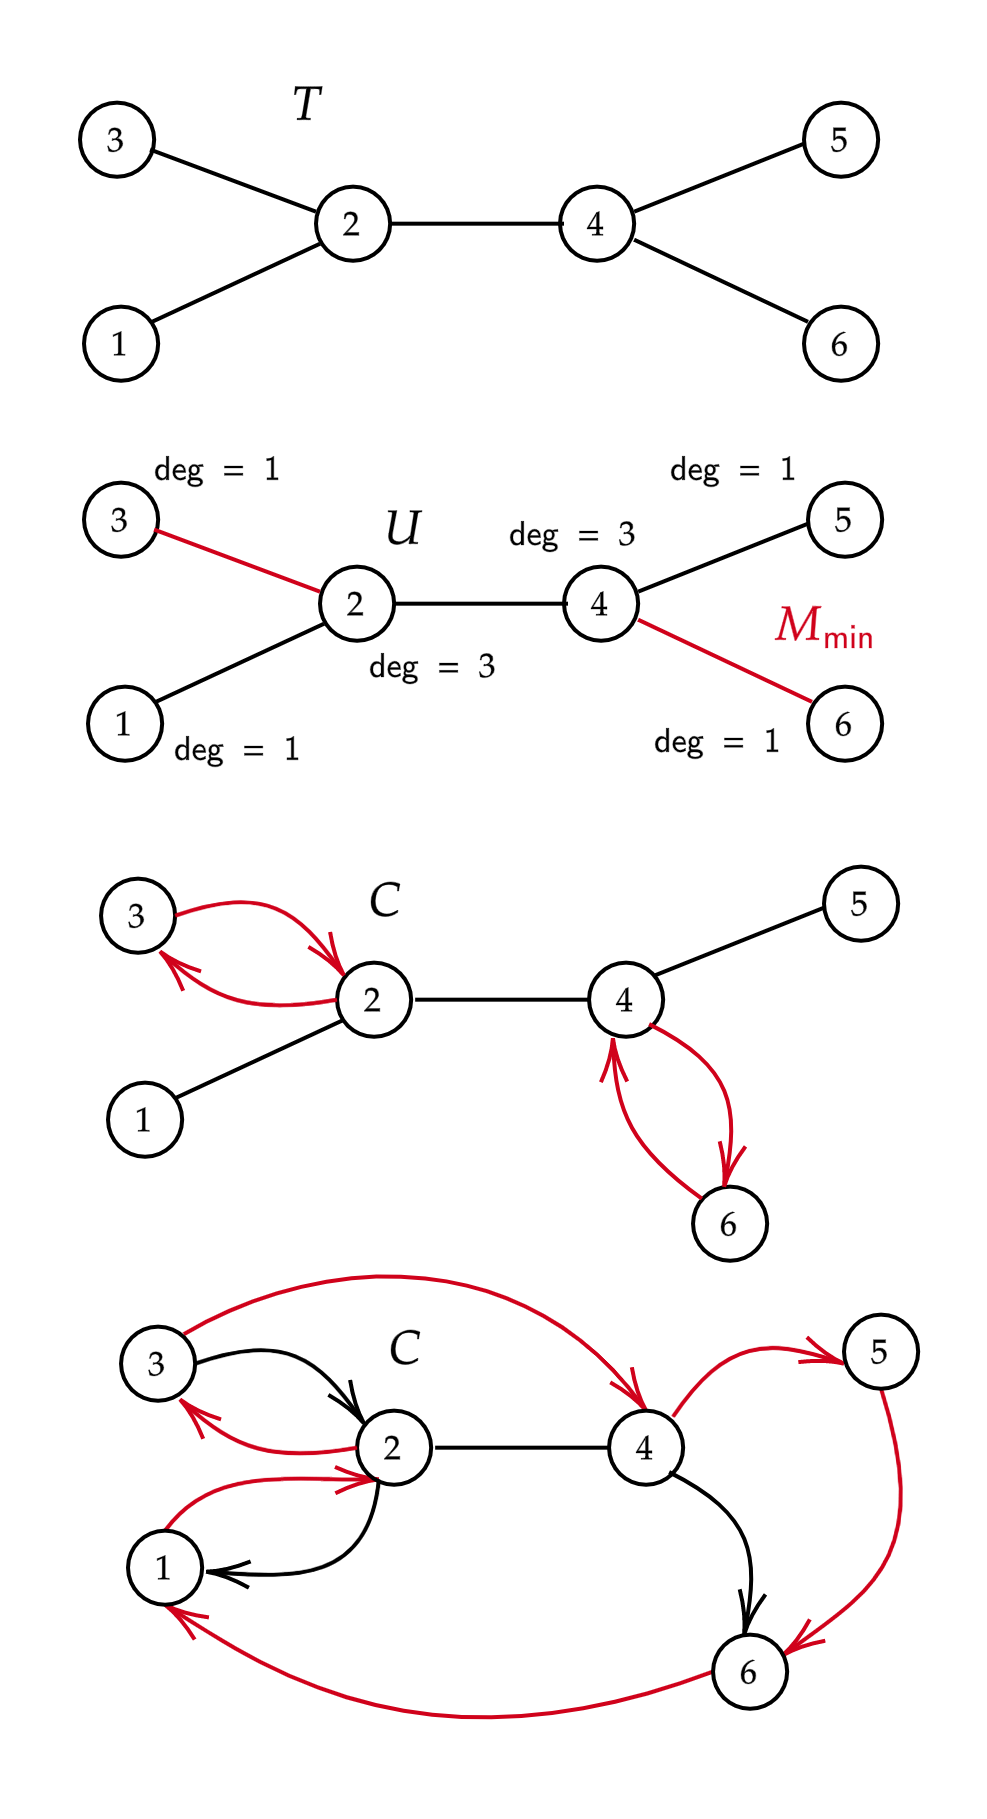
\includegraphics[width=\textwidth]{fig-28.png}
	\caption{Illustration of the \texttt{Christofides} algorithm.}
\end{marginfigure}

\begin{thm}
	There is no polynomial-time $\alpha$-approximation algorithm for the traveling salesman problem on general weighted graphs, unless $P = NP$.
\end{thm}

\begin{proof}
	Construct a cost function for $K_n$ as follows,
	\[
		c(e) := \begin{cases}
						1 & e \in E(G) \\
						\alpha \cdot n& \text{ otherwise}
				   \end{cases}
	\]
	\noindent  Suppose not. If $G$ has a Hamiltonian cycle, then its cost in $K_n$ is $n$. Any other Hamiltonian cycle has cost $\geq \alpha \cdot n + (n - 1) > \alpha n$. Thus, if $G$ has a Hamiltonian cycle, then the $\alpha$-approximation algorithm for the traveling salesman problem must find a tour in $K_n$ of cost $\leq \alpha \cdot n$. The only such tours have cost $n$, and they are Hamiltonian cycles in $G$. This means that the $\alpha$-approximation algorithm can distinguish between \texttt{YES} and \texttt{NO} instances of the Hamiltonian Cycle Problem, which is known to be an NP-complete decision problem.
\end{proof}

\subsection{Application 2: Multiway Cut}
Suppose that we are given an undirected graph \text{$G = (V, E, c)$} with non-negative edge weights $c$, and a set of terminals,
\[X = \{x_1, \cdots, x_k\} \subseteq V(G)\]

\begin{defn}[Multiway Cut]
	A \textbf{multiway cut} is a set of edges that leaves each of the terminals in a separate component\footnote{The Multiway Cut Problem is NP-complete for $k \geq 3$. When $k = 2$, this is precisely finding the minimum $(s - t)$ cut, which can be computed efficiently using \texttt{Ford-Fulkerson}.}.
\end{defn}

\begin{defn}[Multiway Cut Problem]
	The \textbf{Multiway Cut Problem} is the problem of finding a minimum weight set of edges $F \subseteq E(G)$ such that removing $F$ from $G$ separates all terminals\footnote{No connected component of $G(V, E - F)$ contains two terminals from $S$.}.
\end{defn}

\begin{thm}[2-Approximation Multiway Cut]
	The \texttt{MultiApprox} algorithm is a \textbf{2-approximation algorithm} for Multiway Cut.
	\begin{algorithm}
	  \caption{2-Approximation Multiway Cut}\label{2approxMC}
	  \Function{MultiApprox($G$, $c$)}{
	  	\ForEach{$i \in [k]$}{
	  		\Comment{Find a minimum weight cut $\delta(S_i)$ separating $x_i$ from a super-vertex $X_i := X - \{x_i\}$}
	  		$X_i \assign X - \{x_i\}$\;
	  		$C_i \assign \FuncCall{Ford-Fulkerson}{$G$, $c$, $x_i$, $X_i$}$\;
	  	}
	  	\Comment{Return the union of each cut $C_i$}
	  	$C \assign \bigcup_{i = 1}^k \delta(C_i)$\;
	  	\Return{$C$}\;
	  }
	\end{algorithm}
\end{thm}

\begin{proof}
	\texttt{MultiApprox} is a 2-approximation algorithm if,
	\begin{enumerate}
		\item It outputs a feasible cut $C$
		\item It runs in polynomial time
		\item Its cost is at most $2 \cdot \texttt{OPT}$
	\end{enumerate}

	\noindent The cut $C_i$ can be computed efficiently at each iteration by running the \texttt{Ford-Fulkerson} algorithm to find maximum flow. We call a polynomial algorithm a constant number of times, so \texttt{MultiApprox} is polynomial. Moreover, $C = \bigcup_{i = 1}^k \delta(C_i)$ is a feasible multiway cut\footnote{To see this, note that for any pair $x_i, x_j$, $\delta(S_i)$ and $\delta(S_j)$ separate $x_i$ and $x_j$.}. 

	Let \texttt{OPT} denote the optimal multiway cut in $G$. Then $G - \texttt{OPT}$ has components $T_1, \cdots, T_k$, where $x_i \in T_i$. Thus, $\texttt{OPT} = \bigcup_{i = 1}^k \delta(T_i)$ and $c(\texttt{OPT}) = \frac{1}{2} \cdot \sum_i c(\delta(T_i))$ since $e \in \texttt{OPT}$ appears in two of the $\delta(T_i)$,
	\begin{align*}
		c(\texttt{OPT}) &= \frac{1}{2} \cdot \sum_i c(\delta(T_i)) \\
						&\geq \frac{1}{2} \cdot \sum_i c(\delta(C_i)) \\
						&= \frac{1}{2} \cdot c(C) \\
	\end{align*}
	where the second last line follows by the minimality of the cut returned by \texttt{Ford-Fulkerson}, and the last line follows by the union bound. That is, an edge $e \in C$ can appear in only one $\delta(C_i)$ since $C_1 \cup \cdots \cup C_k$ need not equal $V(G)$.
\end{proof}

\subsection{Application 3: Weighted Vertex Cover}
Given a graph $G = (V, E, c)$ and non-negative costs $c$, the goal is to find a minimum cost vertex cover $S \subseteq V(G)$.

\begin{thm}
	The \texttt{GMatching} algorithm is a \textbf{2-approximation algorithm} for the Unweighted Vertex Cover Problem\footnote{The following bound can be seen to be tight by looking at the unweighted vertex cover for a star.}.
	\begin{algorithm}
	  \caption{2-Approximation Vertex Cover}\label{vertcov}
	  \Function{GMatching($G$, $c$)}{
	  	\Comment{Find a maximal cardinality matching $M$ in $G$}
	  	$M \assign \FuncCall{MaxMatching}{$G$}$\;
	  	\Comment{Output $C$, the end vertices of edges in $M$}
	  	$C \assign V(M)$\;
	  	\Return{$C$}\;
	  }
	\end{algorithm}
\end{thm}

\begin{proof}
	\texttt{GMatching} is a 2-approximation algorithm if,
	\begin{enumerate}
		\item It outputs a feasible vertex cover $C$
		\item It runs in polynomial time
		\item Its cost is at most $2 \cdot \texttt{OPT}$
	\end{enumerate}

	\noindent \texttt{GMatching} runs in polynomial time because we can find a maximal matching and its endpoints in polynomial time. Moreover, \texttt{GMatching} outputs a feasible solution because the  maximality of $M$ guarantees that $C$ is a vertex cover of $G$. Since $C^c := V - C$ is an independent set, adding any edge $(i,j) \in E(G - C)$ to $M$ creates a bigger matching.

	We need to show that $|C| \leq 2 \cdot \texttt{OPT}$. Let $C^*$ be the minimum vertex cover in $G$, so that $|C^*| = \texttt{OPT}$. Then $\texttt{OPT} \geq |M|$, where $M$ is the maximal matching in $G$. This is because $C^*$ must contain at least one endpoint of each edge in $M$. But, $|C| = 2 \cdot |M|$, so,
	\[|C| = 2 \cdot |M| \leq 2 |C^*| = 2 \cdot \texttt{OPT}\]
\end{proof}

\begin{marginfigure}
	\textbf{Recall: } A basic solution to a linear program is a feasible solution that is not a convex combination of two other feasible solutions.

	\begin{center}
		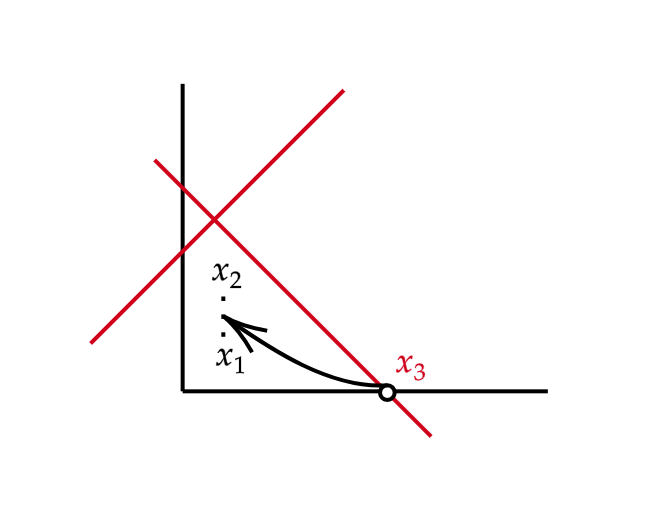
\includegraphics[width=\textwidth]{fig-29.png}
	\end{center}
		
	\noindent \textbf{Recall: } A convex combination is a linear combination of points where all coefficients are non-negative and sum to 1. Moreover, there is always an optimal solution that is basic.
\end{marginfigure}

\begin{thm}
	The \texttt{Rounding} algorithm is a \textbf{2-approximation algorithm} for the weighted Vertex Cover Problem. The integer program is,
	\[
	\begin{array}{lll}
		\operatorname{minimize} & \sum_{i \in V(G)} c_i \cdot x_i & \\
		\text{ subject to } & x_i + x_j \geq 1 & \quad \forall (i, j) \in E(G) \\
		& x_i \in\{0,1\} & \quad \forall i \in V(G)
	\end{array}
	\]
	\noindent but it requires exponential time to solve. Relaxing to a linear program,
	\[
	\begin{array}{lll}
		\operatorname{minimize} & \sum_{i \in V(G)} c_i \cdot x_i & \\
		\text{ subject to } & x_i + x_j \geq 1 & \quad \forall (i, j) \in E(G) \\
		& x_i \in [0,1] & \quad \forall i \in V(G)
	\end{array}
	\]
	\noindent we output $C := \{i \in V \mid x_i \geq \frac{1}{2}\}$.
\end{thm}

\begin{proof}
	\texttt{Rounding} is a 2-approximation algorithm if,
	\begin{enumerate}
		\item It outputs a feasible vertex cover $C$
		\item It runs in polynomial time
		\item Its cost is at most $2 \cdot \texttt{OPT}$
	\end{enumerate}
	\noindent \texttt{Rounding} clearly runs in polynomial time since we have applied relaxation. We need to show that the algorithm outputs a feasible vertex cover. Consider any edge $(i,j) \in E(G)$. By the linear programming constraints, $x_i + x_j \geq 1$, so,
	\[\max\left\{x_{i}, x_{j}\right\} \geq \frac{1}{2}\left(x_{i}+x_{j}\right) = \mu\]
	\noindent and at least one endpoint of $(i,j)$ is in $C$.

	To find the approximation guarantee, let $C^*$ be the minimum cost vertex cover in $G$. $\hat{x}$ is a feasible linear programming solution if\footnote{The optimal solution is feasible.},
	\begin{align*}
	 	\hat{x}_{i}= \begin{cases}1 & i \in C^{*} \\ 0 & i \not\in C^{*}\end{cases}
	 \end{align*}

	\noindent The optimal relaxed linear programming solution $x$ satisfies,
	\[c\left(x\right)=\sum_{i \in V} c_{i} x_{i} \leq \sum_{i \in V} c_{i} x^*_{i} = \texttt{OPT}\]

	\noindent This gives that,
	\begin{align*}
		c(C) &= \sum_{i : x_i \geq 1/2} c_i \\
			 &\leq \sum_{i : x_i \geq 1/2} c_i (2 x_i) \text{ since $2 x_i \geq 1$}\\
			 &\leq 2 \cdot \sum_{i \in V} c_i x_i \\
			 &= 2 \cdot \texttt{OPT}
	\end{align*}
\end{proof}

\begin{thm}
	The linear program for Vertex Cover is $1/2$-integral. That is, any basic solution $\Vec{x}$ satisfies that $x_i \in \{0,1/2,1\}$.
\end{thm}

\begin{proof}
	Let $\Vec{x}$ be a basic solution to our linear program. We can assume that $\Vec{x}$ is fractional, i.e., $0 < x_i < 1$. Suppose not. Then,
	\begin{enumerate}
		\item $x_i = 1$ for some $i \in V$. Select $i \in C$ and consider $G - i$.
		\item $x_i = 0$ for some $i \in V$. Discard $i \in C$ and consider $G - i$\footnote{Any edge with $x_i$ satisfies that its other endpoint is assigned a value of $1$. This follows from the constraints of our integer program, i.e., $x_i + x_j \geq 1$.}
	\end{enumerate}
	\noindent We need to prove that any $x_i$ with a fractional value is $1/2$. 
	\begin{align*}
		V^+ &:= \{i \mid x_i > 1/2\} \\
		V^- &:= \{i \mid x_i < 1/2\} \\
		V^{1/2} &:= \{i \mid x_i = 1/2\} \\
	\end{align*}
	\noindent Observe that $\Vec{x} = \frac{1}{2}(\Vec{y} + \Vec{z})$, where $y_i$ and $z_i$ are defined as follows,
	\[y_{i}=\begin{cases}
			x_{i} & i \in V^{1/2} \\
			x_{i}+\delta & i \in V^{+} \\
			x_{i}-\delta & i \in V^{-}
			\end{cases}
	\quad\quad
	 z_{i} = \begin{cases}x_{i} & i \in V^{1/2} \\
			x_{i}-\delta & i \in V^{+} \\
			x_{i}+\delta & i \in V^{-}\end{cases}\]
	\noindent so $\Vec{x}$ is a convex combination of $\Vec{y}$ and $\Vec{z}$. We will show that $\Vec{y}$ and $\Vec{z}$ are feasible solutions to obtain a contradiction. There can be no edges within $V^-$ or between $V^-$ and $V^{1/2}$ since the constraint $x_1 + x_j \geq 1$ would not be satisfied. The only edges that we can have are,
	\begin{enumerate}
	 	\item $E_1$, between $V^-$ and $V^+$
	 	\item $E_2$, between $V^+$ and $V^{1/2}$
	 	\item $E_3$, within $V^+$ 
	 	\item $E_4$, within $V^{1/2}$
	 \end{enumerate} 
	 \noindent This implies that $\Vec{y}$ is feasible for the linear program,
	 \begin{enumerate}
	 	\item $(i,j) \in E_1$, then $y_i + y_j = (x_i + \delta) + (x_i - \delta) = x_i + x_j \geq 1$
	 	\item $(i,j) \in E_4$, then $y_i + y_j = x_i + x_j \geq 1$
	 	\item $(i,j) \in E_2$, then $y_i + y_j = x_i + (x_j - \delta) = x_i + x_j - \delta \geq 1$
	 	\item $(i,j) \in E_3$, then $y_i + y_j = (x_i - \delta)  + (x_j - \delta) = x_i + x_j - 2\delta \geq 1$
	 \end{enumerate}
	 \noindent since edges in $E_2$ and $E_3$ are such that $x_i + x_j > 1$. Hence, we can choose $\delta$ so that $y_i + y_j \geq 1$. The case for the feasibility of $\Vec{z}$ is analogous. Thus, $\Vec{x} = \frac{1}{2}(\Vec{y} + \Vec{z})$, where $\Vec{y}$ and $\Vec{z}$ are feasible. This is a contradiction unless $\Vec{y} = \Vec{z}$, but then $V^- = V^+ = \emptyset$ so $x_i \in \{0,1/2,1\}$.
\end{proof}

\begin{cor}
	Every basic solution is integral for a bipartite graph.
\end{cor}

\begin{proof}
	Take a basic solution $\Vec{x}$. We proved that $x_i \in \{0,1/2,1\}$, and we can reduce to the case where $\Vec{x}$ is all-fractional. Defining $\Vec{x} = \frac{1}{2}(\Vec{y} + \Vec{z})$, where $y_i$ and $z_i$ and $L, R$ are the bipartitions of $G$,
	\[y_{i}=\left\{\begin{array}{l}
	x_{i}+\delta \quad i \in L \\
	x_{i}-\delta \quad i \in R
	\end{array} \quad z_i =\left\{\begin{array}{l}
	x_{i}-\delta \quad i \in R \\
	x_{i}+\delta \quad i \in L
	\end{array}\right.\right.\]
	\noindent Every edge has one endpoint in $L$ and the other in $R$, 
	\begin{enumerate}
		\item $y_i + y_j = (x_i + \delta) + (x_j - \delta) = x_i + x_j \geq 1$
		\item $z_i + z_j = (x_i - \delta) + (x_j + \delta) = x_i + x_j \geq 1$
	\end{enumerate}
	\noindent implying that $L = R = \emptyset$. Hence, there are no vertices with $x_i = 1/2$. This implies that $\Vec{x}$ is integral, that is, $x_i \in \{0,1\}$.
\end{proof}

\begin{cor}
	Vertex cover is polynomial for a bipartite graph\footnote{We have a 1-approximation algorithm for bipartite graphs.}.
\end{cor}

\begin{thm}
	There is a \textbf{$3/2$-approximation algorithm} for the Vertex Cover Problem in a planar graph.
\end{thm}

\begin{proof}
	Solve the linear program relaxation to obtain a solution $\Vec{x}$ that is $1/2$-integral. Let $V^1 := \{i \mid x_i = 1\}$ and $V^{1/2} := \{i \mid x_i = 1/2\}$. The subgraph of $G$ with vertex set $V^{1/2}$ is planar. By the Four Color Theorem, it can be partitioned into four stable sets, $Q_1, Q_2, Q_3, Q_4$.
	\[V^1 \cup Q_1 \cup Q_2 \cup Q_3\]
	\noindent is a vertex cover\footnote{This effectively takes everything except $V^0$ and $Q_4$, but no edges bridge them by the linear program constraints.}. The linear programming solution is $\sum_{i \in V} c_i \cdot x_i$. Without loss of generality, assume that,
	\[\sum_{i \in Q_4} c_{i} x_{i} \geq \sum_{i \in Q_l} c_{i} x_{i} \quad \quad \forall l=\{1,2,3\}\]
	\noindent But $x_i = 1/2$ for all $i \in \cup_i Q_i$. Hence,
	\[\sum_{i \in Q_4} c_i \geq \sum_{i \in Q_l} c_i \quad \quad \forall l=\{1,2,3\}\]
	\noindent This makes the cost of the algorithm,
	\begin{align*}
	&c(A)=\sum_{i \in V^1} c_{i}+\sum_{i \in Q_1 \cup Q_2 \cup Q_3} c_{i}\\
	&\leq \sum_{i \in V^1} c_{i} \cdot x_{i} + \frac{3}{4} \cdot \sum_{i \in Q_1 \cup Q_2 \cup Q_3 \cup Q_4} c_{i}\\
	&\leq \frac{3}{2} \cdot \sum_{i=V} c_{i} x_{i} \\
	&\leq \frac{3}{2} \cdot \texttt{OPT}
	\end{align*}
	\noindent Thus, we have a $3/2$-approximation algorithm for planar graphs\footnote{The second last inequality follows because the cost of the relaxed program is less than the cost of integer one.}.
\end{proof}

\subsection{Application 4: Set Cover}
We are given $n$ elements $V = \{v_1, \cdots, v_n\}$ and $m$ sets $S_1, \cdots, S_m \subseteq V$ with costs $c_1, \cdots, c_m$. The goal is to find a minimum cost collection of sets that cover every element in $V$. This problem is NP-Complete.

\begin{thm}[Greedy Set Cover]
	\texttt{GreedySet} is a \textbf{$O(\log n)$-approximation algorithm} for the Set Cover Problem. The algorithm is greedy.
\end{thm}

\begin{algorithm}
	  \caption{Greedy Algorithm for Set Cover}\label{setcovergreedy}
	  \Function{GreedySet($X$, $S$)}{
	  \Comment{$U$ stores the uncovered elements}
	  $U \assign X$\;
	  \Comment{$C$ stores the sets of the cover}
	  $C \assign \emptyset$\;
	  \While{$U \neq \emptyset$}{
	  		\Comment{Select the set $S_j^*$ which covers the remaining uncovered elements at a minimum average cost}
		  	$S_j \assign S_j^*$\;
		  	$C \assign C \cup S_j$\;
		  	$U \assign U - S_j^*$\;
	  	}
	    \Return{$C$}\;
	  }
\end{algorithm}

\begin{marginfigure}
	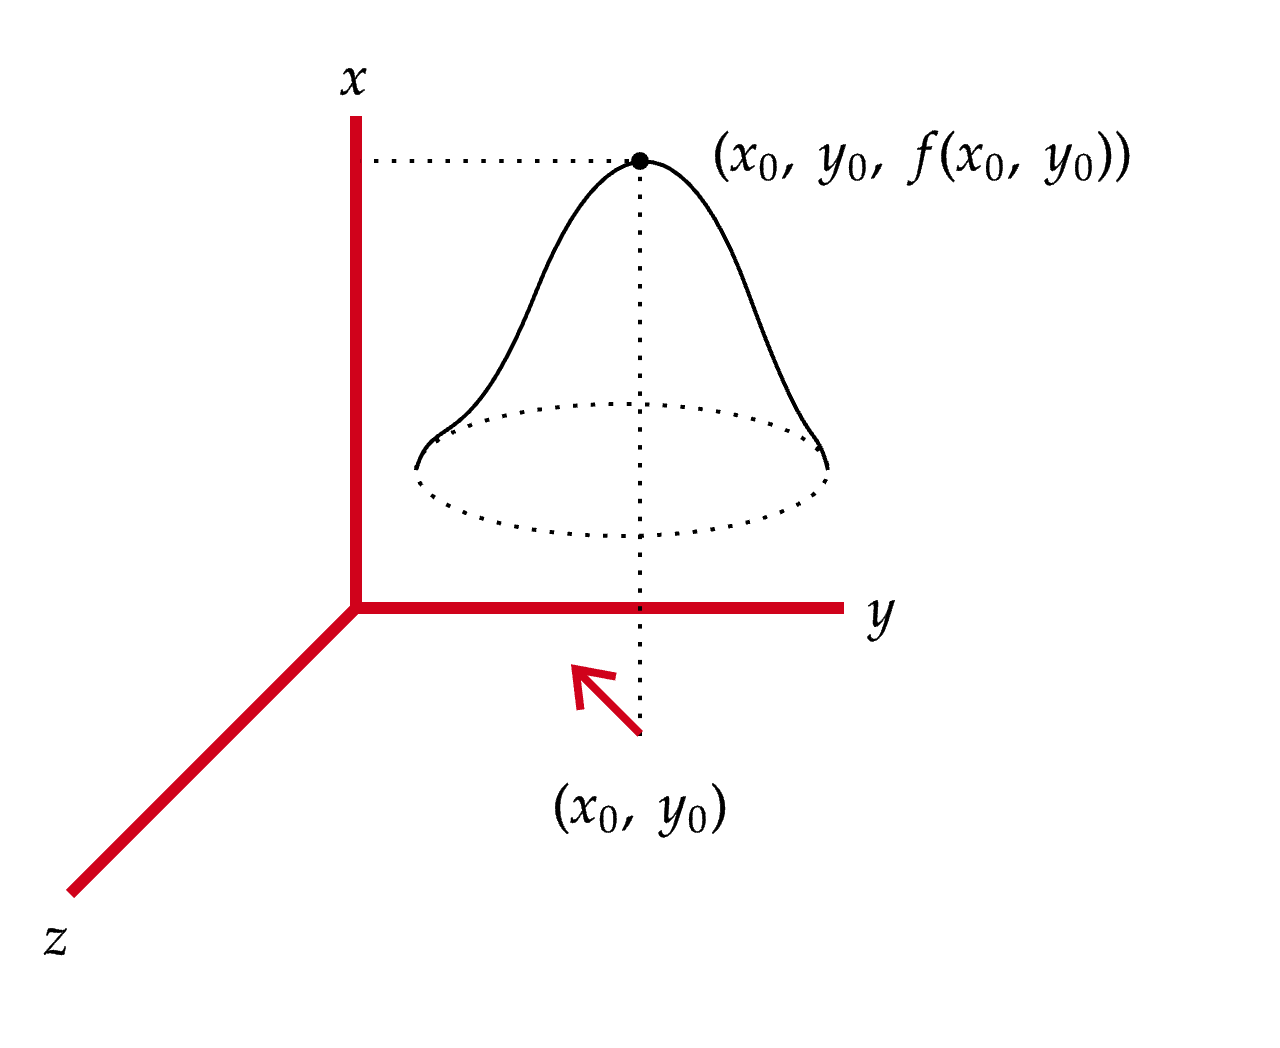
\includegraphics[width=\textwidth]{fig-30.png}
	\caption{Illustration of \texttt{GreedySet}. Sets are sorted by average cost, where the average is taken over cardinality.}
\end{marginfigure}

\begin{proof}
	The algorithm clearly runs in polynomial time and outputs a feasible set cover. We need to prove that $\alpha = O(\log n)$. Let,
	\begin{align*}
		&\texttt{OPT} := \{S^*_1, \cdots, S_k^*\}
		&\underbrace{C := \{S_1, \cdots, S_r\}}_{r \text{ possibly } \neq k}
	\end{align*}
	\noindent and $C$ as the output of \texttt{GreedySet}. We want to prove that,
	\[\sum_{j=1}^r c(S_j) \leq \log n \cdot \sum_{j=1}^k c(S_j^*)\]

	Label the elements of $V$ by $\{1, 2, \cdots, n\}$, based on the order that they are covered by \texttt{GreedySet}. Let $U_t$ be the set of uncovered elements at the start of step $t$\footnote{$U_1 = V$ and $U_t \subset U_{t-1}$.}. If $S_t$ is the set selected by \texttt{GreedySet} at $t$, then $n_t = |S_t \cap U_t|$ is the number of new elements covered at $t$.

	\noindent If $i \in S_t \cap U_t$, then $i$ was covered at step $t$. Then,
	\[\alpha_i = \frac{c(S_t)}{n_t}\]

	\noindent is the cost of covering $i$. Hence, $\sum_{t=1}^{k} c(S_{t})=\sum_{i=1}^{n} \alpha_{i}$. To see this,
	\begin{align*}
		\sum_{t=1}^{r} c(S_{t}) &= \sum_{t=1}^{r} \alpha_i \cdot n_t \\
								&= \sum_{i=1}^{n}  \alpha_i \quad \text{(where $|V| = n$)}\\
	\end{align*}

	To analyze the cost of \texttt{GreedySet}, it suffices to bound $\alpha_i$. When $i$ was covered, there were at least $n - i + 1$ uncovered elements. \texttt{OPT} can cover all of these elements for an average cost of,
	\[\frac{1}{n-i+1} \cdot \left(\sum_{i=1}^{k} c(S_i^*)\right)=\frac{1}{n-i+1} \cdot \texttt{OPT}\]

	Since $S_t$ must do at least as well as this, $\alpha_i \leq \frac{1}{n-i+1} \cdot \texttt{OPT}$,
	\begin{align*}
		\sum_{i=1}^{n}  \alpha_i &\leq \sum_{i=1}^{n} \frac{1}{n-i+1} \cdot \texttt{OPT} \\
								 &= \texttt{OPT} \cdot \sum_{i=1}^{n} \frac{1}{n-i+1} \\
								 &= \texttt{OPT} \cdot \sum_{l=1}^n \frac{1}{l} \\
								 &= \texttt{OPT} \cdot H_n
	\end{align*}
	\noindent where $H_n \approx \log n$ is the $n$th partial sum of a Harmonic series. Thus,
	\[c(\{S_1, \cdots, S_r\}) \leq O(\log n) \cdot \texttt{OPT}\]
\end{proof}

\begin{ex}{Proof of Tighteness}{label}
	Suppose that all sets have cost \$1. Then,
	\begin{align*}
		&c(\texttt{OPT}) = c(\{S_1^*, S_2^*\}) = 2\\
		&c(C) = c(\{S_1, \cdots, S_r\}) =  r
	\end{align*}
	\begin{center}
		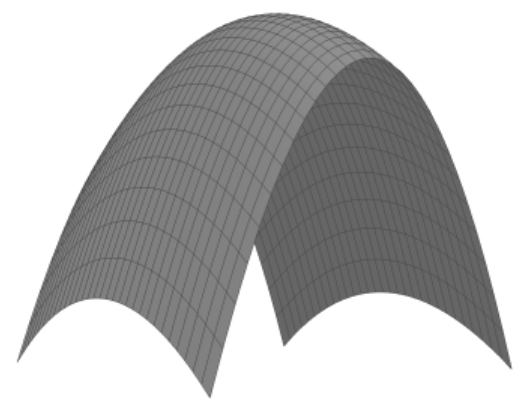
\includegraphics[width=\textwidth]{fig-31.png}
	\end{center}
	\noindent But, $r = \Omega\left(\log n \right)$ so $n = 2 + \sum_{j=1}^{r-1} 2^j$.
\end{ex}

\begin{rmk}
	There is no $\alpha$-approximation for the Set Cover Problem with $\alpha = c \cdot \log n$ and $c < 1$ unless $P = NP$. We will not see the proof of this.
\end{rmk}

\subsection{Application 5: Hitting Set}
We are given $m$ elements $E = \{1, 2, \cdots, m\}$ with respective costs $c_1, c_2, \cdots, c_m$ and sets $T_1, T_2, \cdots T_n \subseteq E$. The goal is to find a minimum cost set of elements that "hit" every set $T_1, \cdots, T_n$.

\begin{rmk}
	Since the Hitting Set Problem is equivalent to the Set Cover Problem, we can use \texttt{GreedySet} to solve it.
\end{rmk}

\begin{defn}[Randomized Rounding]
	Let $T_j$ be the indices of the sets $S_j$ that cover element $i$. The integer problem to solve Hitting Set uses a randomized rounding algorithm,
		\[
		\begin{array}{lll}
			\operatorname{minimize} & \sum_{j=1}^m c_i \cdot x_i & \\
			\text{ subject to } & \sum_{j \in T_i} x_j \geq 1 & \quad \forall T_i\\
			& x_i \in\{0,1\} & \quad \forall i \in V(G)
		\end{array}
		\]
	\noindent and it can be relaxed as follows,
	\[
		\begin{array}{lll}
			\operatorname{minimize} & \sum_{j=1}^m c_i \cdot x_i & \\
			\text{ subject to } & \sum_{j \in T_i} x_j \geq 1 & \quad \forall T_i\\
			& x_i \in [0,1] & \quad \forall i \in V(G)
		\end{array}
	\]
	\noindent where element $j$ is selected with probability $x_j$.
\end{defn}

\begin{rmk}
	The expected cost of the randomized algorithm is,
	\[\sum_{j=1}^{m} c_{j} x_{j} = \texttt{LP} \leq \texttt{OPT}\]
	\noindent where \texttt{LP} is the value of our linear program. While the algorithm is polynomial, it may not output a feasible solution.
\end{rmk}

\begin{marginfigure}
	\textbf{Arithmetic-Mean Inequality: }

	\noindent For any $\alpha_1 \cdots \alpha_k \geq 0$,
	\[\frac{\sum_{i} \alpha_{i}}{k} \geq \sqrt[k]{\pi \alpha_{i}}\]
\end{marginfigure}

\begin{rmk}
	If $X_i$ be the event that $T_i$ is hit, then $P(X_i) \geq 1 - \frac{1}{e}$.
\end{rmk}

\begin{proof}
	Put $T_i := \{1, 2, \cdots, k\}$. By the linear programming constraints, $\sum_{j=1}^k x_j \geq 1$. Hence, the probability that $T_i$ is missed is,
	\begin{align*}
		P(X_i^c) &= \prod_{j=1}^k (1 - x_j) \\
				 &= \prod_{j=1}^k \alpha_j \\
				 &\leq \left(\frac{1}{k} \cdot (\alpha_1 + \cdots + \alpha_k\right)^k \\
				 &= (1 - \frac{1}{k} \cdot \sum x_j)^k \\
				 &\leq (1 - \frac{1}{k})^k \text{ since $\sum x_j \geq 1$}
	\end{align*}
	\noindent But, $(1 - \frac{1}{k})^k \leq \frac{1}{e} = \lim_{n \rightarrow \infty} \left(1 - \frac{1}{n}\right)^n$. Thus, the probability that $T_i$ is hit is strictly bigger than $\frac{1}{2}$.
\end{proof}

\begin{cor}
	Our solution may miss half the sets. If the algorithm is run $\ell = 2 \log n$ times, then the probability of missing a set is reduced to $\frac{1}{n}$\footnote{Consequently, with high probability, randomized rounding gives a hitting set with cost $\leq 2 \log n \cdot \texttt{OPT}$.}.
\end{cor}

\subsection{Application 6: Maximum Satisfiability}
Let $x_1, x_2, \cdots, x_n$ be boolean variables. Recall that,
\begin{enumerate}
	\item A positive literal is a variable $x_i$
	\item A negative literal is a negation $\bar{x_i}$.
	\item A clause is a disjunction of literals
\end{enumerate}
The goal is to assign the variables \texttt{True} and \texttt{False} while satisfying as many as clauses possible.

\begin{thm}
	Independently assigning each variable $x_i$ to be \texttt{True} with probability $1/2$ is a $1/2$-approximation algorithm.
\end{thm}

\begin{proof}
	Take a clause $C_j$ with $k$ literals. $C_j$ is not satisfied with probability $\frac{1}{2^k}$. Therefore, $C_j$ is satisfied with probability $1 - \frac{1}{2^k}$. The worst case occurs when $k = 1$, but $1 - \frac{1}{2^k} \geq \frac{1}{2}$. This means that each clause is satisfied with a probability of at least $\frac{1}{2}$. Let $m$ be the total number of clauses. By linearity of expectation, the expected number of satisfied clauses is at least $\frac{1}{2} \cdot m \geq \frac{1}{2} \cdot \texttt{OPT}$.
\end{proof}

\begin{rmk}
	This is a $7/8$-approximation algorithm for Maximum 3-SAT because each clause is satisfied with probability $1 - \frac{1}{2^3} = \frac{7}{8}$\footnote{In fact, unless P = NP, there is no better approximation algorithm.}.
\end{rmk}

\begin{thm}[Randomized Satisfiability]
	The following integer program solves the Maximum Satisfiability Problem,
	\[
		\begin{array}{lll}
			\operatorname{maximize} & \sum_{j=1}^m z_i & \\
			\text{ subject to } & \sum_{x_i \in C_j} y_j + \sum_{x_i \in C_j} (1 - y_i) \geq z_j & \quad \forall j\\
			& y_i, z_j\in\{0,1\} & \quad \forall i, j
		\end{array}
	\]
	\noindent where clauses are indexed by $j$, variables are indexed by $i$, and each clause $C_j$ corresponds to $z_j$. To see that this works\footnote{The clause constraint is satisfied if and only if at least one of the literals are assigned correctly.}, let, 
	\[
	y_{i}=\left\{\begin{array}{ll}
	1 & \text { if } x_{i}=\texttt{True} \\
	0 & \text { if } x_{i}=\texttt{False}
	\end{array} \quad z_{j}= \begin{cases}1 & \text { if } C_{j} \text { satisfied } \\
	0 & \text { if } C_{j} \text { not satisfied }\end{cases}\right.
	\]
	\noindent We solve the linear program relaxation in polynomial time with $0 \leq y_i \leq 1$ and $0 \leq z_i \leq 1$ for all $i, j$. To do this, set $x_i = \texttt{True}$ with probability $y_i$.
\end{thm}

\begin{marginfigure}
	\textbf{Recall: } If $f(x)$ is concave on $[0,1]$ with $f(0) = t$ and $f(1) = a + b$, then, \[f(x) \geq ax + b\]
\end{marginfigure}

\begin{proof}
	Since $C_j$ has $k$ literals, it is satisfied with minimum probability,
	 \[\left(1 + \left(1 + \frac{1}{k}\right)^k\right) \cdot z_j\]
	 \noindent We will prove this using the Arithmetic Mean Inequality. Without loss of generality, let $C_j \ x_1 \lor x_2 \lor \cdots \lor x_k$. Then,
	\begin{align*}
		\prod_{j=1}^k (1 - y_i) &\leq \left(\frac{\sum (1-y_i)}{k} \right)^k \text{ by the Arithmetic Mean Inequality}\\
								&= \left(1 - \frac{\sum y_i}{k}\right)^k \\
								&\leq \left(1 - \frac{z_j}{k}\right)^k \text{ by the constraint $\sum_{x_i \in C_j} y_i \geq z_j$}
	\end{align*}
	\noindent is the probability that $C_j$ is not satisfied. Note that $g(x) = \left(1 - \frac{x}{k}\right)^k$ is convex, and consequently $f(x) = 1 - g(x)$ is concave. Thus,
	\begin{enumerate}
		\item $f(0) = (1 - 0)^k = 0 = b$
		\item $f(1) = (1 - \frac{1}{k})^k = a + b = a$ since $b = 0$
	\end{enumerate}
	\noindent Hence, the probability that $C_j$ is satisfied is greater than,
	\[a \cdot z_j = \left(1 - \frac{1}{k}\right)^k \cdot z_j\]
	\noindent but we have seen that this gives a guarantee of $\frac{1}{e}$. Thus,
	\[\geq \underbrace{\left(1 - \frac{1}{e}\right)}_{\approx 0.632} \cdot z_k\]
	\noindent The expected number of clauses satisfied is greater than or equal to,
	\[\sum_j 0.632 \cdot z_j \geq 0.632 \cdot \sum_j z_j \geq 0.632 \cdot \sum_j \texttt{OPT}\]
	\noindent since $\sum_j z_j$ is our objective function.
\end{proof}

\begin{thm}
	Taking the best out of the previous two approximation algorithms, $\mathcal{R}_1$ and $\mathcal{R}_2$, gives a $3/4$-approximation algorithm.
\end{thm}

\begin{proof}
	Let $N_1$ and $N_2$ be the number of clauses satisfied by $\mathcal{R}_1$ and $\mathcal{R}_2$, respectively. Simplifying and applying induction with,
	\begin{align*}
		\mathbb{E}[\max \{N_1, N_2\}] &\geq \mathbb{E}\left[\frac{1}{2} \cdot (N_1 + N_2)\right] \text{ since $\max \geq \mu$}\\
								     &= \frac{1}{2} \cdot \mathbb{E}[N_1] + \mathbb{E}[N_2] \text{ by linearity of expectation}
	\end{align*}
	\noindent gives the result. The complete proof is not shown.
\end{proof}

\begin{rmk}
	In fact, we can get a $3/4$ guarantee using non-linear randomized rounding. We solve the linear program to find $y_i$ and $z_i$, and set $x_i = \texttt{True}$ with probability $f(y_i)$. This works if the function $f$ satisfies,
	\[1 - \frac{1}{4^y} \leq f(y) \leq f^{y-1}\]
\end{rmk}

\begin{proof}
	The probability that $C_j$ is satisfied is,
	\begin{align*}
	1-\prod_{x_{i} \in C_{j}}\left(1-f\left(y_{i}\right)\right) \cdot \prod_{\bar{x}_{i} \in C_{j}} f\left(y_{i}\right)
	&\geq 1-\prod_{x_{i} \in C_{j}}\left(1-\left(1-\frac{1}{4 y_{i}}\right)\right) \cdot \prod_{\bar{x}_{i} \in C_{j}} 4^{y_{i}-1} \\
	&=1-\prod_{x_{i} \in C_{j}} \frac{1}{4 y_{i}} \cdot \prod_{\bar{x}_{i} \in C_{j}} 4^{y_{i}-1}\\
	&=1-4^{-\sum_{x_{i} \in C_{j}} y_{i}+\sum_{\bar{x}_{i} \in C_{j}}\left(y_{i}-1\right)}\\
	&=1-4^{-\left(\sum_{x_{i} \in C_{j}} y_{i}+\sum_{\bar{x}_{i} \in C_{j}}\left(1-y_{i}\right)\right)}\\
	&\geq 1 - 4^{2j} \text{ by our constraints}
	\end{align*}
	\noindent Using concavity, $f(z_j) \geq \frac{3}{4} \cdot z_j$.
\end{proof}

\begin{ex}{Proof of Tightness}{label}
	This analysis is tight with respect to the upper bound,
	\begin{enumerate}
		\item $C_1 = x_1 \lor x_2$
		\item $C_2 = x_1 \lor \bar{x}_2$
		\item $C_3 = \bar{x_1} \lor x_2$
		\item $C_4 = \bar{x_1} \lor \bar{x_2}$
	\end{enumerate}

	Moreover, it is tight with respect to \texttt{OPT},
	\begin{enumerate}
		\item $C_1 = x_1 \lor x_2$
		\item $C_2 = x_1 \lor \bar{x_2}$
		\item $C_3 = \bar{x_1} \lor x_2$
		\item $C_4 = \bar{x_1} \lor \bar{x_3}$
	\end{enumerate}
\end{ex}

\subsection{Application 7: Steiner-Tree Problem}
\begin{defn}[Steiner-Tree Problem]
	Suppose that we are given a graph $G = (V, E)$ with edge costs $c_e \geq 0$ and a set $R \subseteq V$ of terminals. The goal is to find a minimum cost subgraph $T$ that connects all the terminals. This subgraph is called a \textbf{Steiner tree}. The non-terminals are called \textbf{Steiner nodes}, and they are only used if they reduce the cost of the tree\footnote{Remark that the leaves of a Steiner tree are necessarily terminals.}.
\end{defn}

\begin{cor}
	If $R = V(G)$, then this is the minimum spanning tree problem. If $R \subset V(G)$, then the problem is NP-Complete.
\end{cor}

 \begin{thm}
 	\texttt{SteinerApprox} is a 2-approximation algorithm.
 \end{thm}

\begin{algorithm}
	  \caption{2-Approximation Algorithm for Steiner Trees}\label{steineralgo}
	  \Function{SteinerApprox($X$, $S$)}{
	  \Comment{For terminals $r_1, r_2$, let $P_{ij}$ be the shortest path between them. Denote its length by $\ell_{ij}$}
	  $P_{ij} \assign \delta(i,j)$\;
	  \Comment{Construct an auxiliary graph $H$ that is a complete graph on the set of terminals. Let $(i,j) \in H$ have cost $\ell_{ij}$}
	  $T \assign \FuncCall{Prim}{$H$, $\ell$}$\;
	  \Return{$\bigcup_{(i,j) \in T} P_{ij}$}\;
	  }
\end{algorithm}

% https://courses.cs.duke.edu/cps296.5/current/scribing/cps590_lec16-17.pdf

 \begin{proof}
 	\texttt{SteinerApprox} is a 2-approximation algorithm if,
	\begin{enumerate}
		\item It outputs a feasible vertex cover $C$
		\item It runs in polynomial time
		\item Its cost is at most $2 \cdot \texttt{OPT}$
	\end{enumerate}
	\noindent \texttt{SteinerApprox} is polynomial, and it outputs a feasible solution. Let $T^*$ be the optimal Steiner tree. We can walk around the outside of $T^*$ to create a circuit $C$. This circuit can be divided into paths,
	\[C = Q_1 \cup Q_2 \cup \cdots \cup Q_k\]
	\noindent where $Q_i$ is the path from $r_i$ to $r_{i+1}$. Thus,
	\[c(C) = 2 \cdot c(T^*) = \sum_{i=1}^k c(Q_i)\]
	\noindent but the path $P = \{r_1, \cdots, r_k\}$ is a spanning tree in $H$. Thus,
	\begin{align*}
		c(F) &\leq c(P) \\
			 &= \sum_{i=1}^{k-1} \ell_{i,i+1} \\
			 &\leq \sum_{i=1}^{k-1} Q_i \\
			 &\leq \sum_{i=1}^k c(Q_i) \\
			 &= 2 \cdot \texttt{OPT}
	\end{align*}
	\noindent Since we return $T^{\prime} = \bigcup_{(i,j) \in T} P_{ij}$, we have,
	\[C(T^{\prime}) \leq c(F) \leq 2 \cdot \texttt{OPT}\]
 \end{proof}

\subsection{Application 8: Knapsack Problem}
Suppose that we are given a bag with capacities $w$ and $n$ objects, where each object $i$ has weight $w_i$ and value $v_i$. The goal is to find the subset of items of maximum value that fit in the Knapsack. We saw that this can be formulated as an integer program,
\[\begin{array}{ll}
		\operatorname{maximize} & \sum_{i=1}^{n} v_{i} \cdot x_{i} \\
		\text{ subject to } & \sum_{i=1}^{n} w_{i} \cdot x_{i} \leq W \\
		& x_{i} \in\{0,1\} \quad \forall i \in[n]
\end{array}\]

\begin{lem}
	For a basic solution $\Vec{x}$, there is at most one item with,
	\[0 < x_i < 1\]
\end{lem}

\begin{proof}
	Recall the Greedy Algorithm for the Knapsack Problem,
	\begin{enumerate}
		\item Compute the value per weight $V_i := v_i / w_i$ for each item
		\[\frac{v_1}{w_1} \geq \frac{v_2}{w_2} \geq \cdots \geq \frac{v_n}{w_n}\]
		\item Iterating through the sorted list, put,
		\[
		x_i^G = \begin{cases}
			1 & \text{if $i$ fits completely} \\
			0 & \text{if the knapsack is full} \\
			\frac{W - \sum_{l=1}^{i-1} w_l}{w_i} & \text{otherwise}
		\end{cases}
		\]
	\end{enumerate}
	\noindent After the first fractional item $0 < x_k^G < 1$, the bag is full. Thus,
	\begin{align*}
		\Vec{x}^G &= \left(x_1^G, \cdots, x_{k-1}^G, x_k^G, x_{k+1}^G, \cdots x_n^G\right) \\
				  &= \left(1, \cdots, 1, 1, x_k^G, \cdots 0, \cdots, 0\right)
	\end{align*}
	\noindent An exchange argument shows that $\Vec{x}^G$ is the optimal solution. Assume for a contradiction that it is not. Then some items before $k$ are used below 1. Re-assign weight from $x_j$ to $x_i$, where $i < k \leq j$ by setting,
	\begin{align*}
		&x_j \leftarrow x_j - \delta \\
		&x_i \leftarrow x_i + \frac{\delta \cdot w_j}{w_i}
	\end{align*}
	to save $\delta \cdot w_j$ in weight. The change in value is,
	\[-\delta \cdot v_{j}+\delta \cdot \frac{w_{j}}{w_{j}} \cdot v_{i}=\delta \cdot w_{j} \cdot\left(\frac{v_{i}}{w_{i}}-\frac{v_{i}}{w_{j}}\right) \geq 0\]
	\noindent as $i$ has a better "bang-for-buck" than $j$. We can repeat this until we obtain $\Vec{x}^G$, but this means that $\Vec{x}^G$ is an optimal basic solution\footnote{The solution is basic because it only has one fractional value.}.
\end{proof}

\begin{rmk}
	This gives the following polynomial \texttt{BestOfTwo} algorithm,
	\begin{enumerate}
		\item Solve the linear programming relaxation
		\item Output the maximum value subset between,
		\[I_1 := \{i \mid x_i = 1\} \quad I_2 := \{i \mid 0 < x_i < 1\}\]
	\end{enumerate}
	\noindent where $I_1$ and $I_2$ are both feasible solutions,
	\begin{enumerate}
		\item $I_1$ is feasible since it has weight $\leq W$
		\item $I_2$ is feasible since each weight is less than the size of the bag\footnote{If not, then we can remove this item and recurse to obtain a solution with the same properties.}
	\end{enumerate}
\end{rmk}

\begin{proof}
	\texttt{BestOfTwo} is a 2-approximation algorithm because,
	\begin{align*}
		\max \{v(I_1), v(I_2)\} &\geq \frac{1}{2} \cdot \left(v(I_1) + v(I_2)\right) \\
								&= \frac{1}{2} \sum_{i=1}^n v_i \\
								&\geq \frac{1}{2} \sum_{i=1}^n v_i \cdot x_i \\
								&\geq \frac{1}{2} \cdot \texttt{OPT}
	\end{align*}
\end{proof}

\begin{defn}[Approximation Scheme]
	An algorithm $\mathcal{A}$ is a \textbf{fully polynomial time approximation scheme} for a maximization problem if, 
	\begin{enumerate}
		\item $\mathcal{A}$ outputs a solution of value $\geq (1 - \epsilon) \cdot \texttt{OPT}$
		\item $\mathcal{A}$ runs in time polynomial in $|\texttt{I}|$ and $\frac{1 }{\epsilon}$
	\end{enumerate}
	\noindent for any instance \texttt{I} and $\epsilon > 0$.
\end{defn}

\begin{thm}
	There is a fully polynomial time approximation scheme for the Knapsack Problem. It is based on dynamic programming.
\end{thm}

\begin{proof}
	Let $w(i, V)$ be the minimum weight of a subset of the items $[i]$ of value $\geq V$. This is by convention infinite if the value of $[i]$ is less than $V$. The dynamic program can be solved recursively as $w(i, V) = \min \{w(i-1,V), w_i + w(i-1, V - v_i)\}$ with base cases $w(i, V) = 0$ for all $V \leq 0$. Let $V_{\max} := \max_i v_i$. Then there are $n$ choices for $i$ and at most $n \cdot V_{\max}$ choices for $V$. This means that there are $O(n^2 \cdot V_{\max})$ subproblems, solvable in $O(2)$.

	Since $V_{\max}$ can be exponential in the number of bits, this is a pseudo-polynomial time algorithm. We can resolve this by scaling down each value without substantially losing accuracy. 
\end{proof}

\subsection{Parameterized Complexity}
\begin{defn}[Fixed-Parameter Tractable]
	A problem is \textbf{fixed parameter tractable} if it has an algorithm to solve it that runs in time $f(k) \cdot \text{poly}(n)$, where $n$ is the problem input size, $k$ is the size of the optimal solution, and $f$ need not be a polynomial function.
\end{defn}

\begin{ex}{Vertex Cover}{label}
	If we are given that the optimal solution $C^*$ to the Vertex Cover Problem has \text{$k$} vertices, then we can check in \text{$O\left(m \cdot \binom{n}{k}\right) = O(m \cdot n^k)$} if a subset \text{$C$} is a vertex cover.

	This running time is exponential in the size of the optimal solution, not in the input size. It serves as a motivating example for the question: \textit{Can we separate the time dependency on $n$ and $k$ completely?} Specifically, we want an algorithm in,
	\[O(\text{poly}(n) \cdot f(k))\]
	\noindent where $f(k)$ is exponential, or worse, in $k$. If we can do this, then the problem is called \textbf{fixed parameter tractable}.
\end{ex}

\begin{lem}
	Let $M^*$ be a maximum matching and $C^*$ be a minimum vertex cover in a non-bipartite graph. Then,
	\[\left|M^{*}\right| \leq\left|C^{*}\right| \leq 2 \cdot\left|M^{*}\right|\]
\end{lem}

\begin{proof}
	Let $M^* := \{e_1, e_2, \cdots, e_l\}$, where $e_i = (u_i, v_i)$. Then $V - V(M^*)$ is an independent set in $G$\footnote{If not, then we could construct a larger matching than $M^*$.}. Moreover, $V(M^*)$ is a vertex cover. This means that the minimum vertex cover $C^*$ is at most the size of $C$,
	\[\left|C^{*}\right| \leq|C|=2 \cdot l=2 \cdot\left|M^{*}\right|\]
\end{proof}

\begin{thm}
	% Vertex Cover is fixed-parameter tractable.
	Let $G$ be a non-bipartite graph with minimum vertex cover $C^*$ of size $k$. Then, $C^*$ can be found in time $3^k \cdot \text{poly}(n)$.
\end{thm}

\begin{proof}
	Find a maximum matching $M^* = \{e_1, \cdots, e_l\}$ in polynomial time. Observe that $l \leq k$, or else $|C^*| \geq k$. At least one endpoint $e_i = (u_i, v_i)$ is in $C^*$, so there are three possibilities for $e_i$,
	\begin{align*}
		&u_{i} \in C^{*} \wedge v_{i} \notin C^{*} \\
		&u_{i} \notin C^{*} \wedge v_{i} \in C^{*} \\
		&u_{i} \in C^{*} \wedge v_{i} \in C^{*}
	\end{align*}
	\noindent This gives $3^l$ possibilities, producing subsets $C_1, \cdots, C_{3^l}$. Moreover, we know that there exists $j$ such that $C_j = C^* \cap V(M^*)$. To find the correct index $j$, we can try every possibility. There are two cases,
	\begin{enumerate}
		\item There is an edge $e$ whose endpoints are both in $V(M^*) - C_j$. Then it cannot be covered by adding vertices of $V - M^*$ to $C_j$. Thus, this is not the correct choice and we can reject it.
		\item There are no edges whose endpoints are both in $V(M^*) - C_j$. Any edge $e$ incident to a vertex in $C_j$ is already covered. Since $V - M^*$ is an independent set, any other edge $f$ has one endpoint in $V(M^*) - C_j$ and the other in $V - V(M^*)$. To cover these edges, we select a vertex in $V - V(M^*)$ as $C_j$ are the only vertices in $V(M^*)$ that touch at least one edge uncovered by $C_j$. Let $W_j$ be the set of vertices in $V - V(M^*)$ that touch at least one edge uncovered by $C_j$. Thus, $\hat{C}_j = C_j \cup W_j$ is the smallest vertex cover $C$ such that,
		\[\hat{C}_j = C_j \cup W_j\]
		\noindent We output the smallest $\hat{C}_j$, which is the minimum vertex cover.
	\end{enumerate}
	We conclude that the total running time is at most,
	\[3^l \cdot \text{poly}(n) \leq 3^k \cdot \text{poly}(n)\]
\end{proof}

We can repeat the same procedure for the Longest Path Problem.

\begin{thm}
	Suppose that the longest path $P^*$ contains exactly $k$ vertices,
	\[P^* = \{v_1, v_2, \cdots, v_k\}\]
	\noindent We can find $P^*$ exhaustively in $O(k \cdot n^k)$ by,
	\begin{enumerate}
		\item Taking every possible sequence $P$ of $k$ vertices
		\item Testing if $P$ is a path
	\end{enumerate}
\end{thm}

In fact, we can do better. A useful technique in the design of fixed parameter tractable algorithms is the color coding method.

\begin{defn}[Color Coding]
	The \textbf{color coding method} colors each object in the search space, so that the algorithm can refine its search for monochromatic or panchromatic solutions.
\end{defn}

\begin{rmk}
	The color coding method applies to the Longest Path Problem.
\end{rmk}

\begin{proof}
	Assume the longest path is $P^* = \{v_1, v_2, \cdots, v_k\}$. Randomly color the vertices of $G$ with $k$ colors. If col($v_i$) $= i$ for all $1 \leq i \leq k$, then we can find $P^*$ in linear time by Breadth-First Search:
	\begin{enumerate}
		\item Begin with vertices of color 1, and search for neighbors in color 2
		\item From these neighbors, search for neighbors of neighbors of color 3
		\item Repeat this procedure until color $k$
	\end{enumerate}
	\noindent The probability that $v_i$ is given color $i$ is $\frac{1}{k}$, so the probability that every vertex in $P^*$ is given the correct color is,
	\[\left(\frac{1}{k}\right)^k\]
	Suppose that the color coding algorithm is run $t$ times. Each run is independent, so the probability of failure every time is at most,
	\[\left(1-\left(\frac{1}{k}\right)^{k}\right)^{t}=\left(1-\frac{1}{k^{k}}\right)^{t}\]
	\noindent Using the fact that $1-x<e^{-x} \quad \forall x \neq 0$,
	\[\left(1-\frac{1}{k^{k}}\right)^{t} \leq\left(e^{-\frac{1}{k^{k}}}\right)^{t}=e^{-\frac{t}{k^{k}}}\]
	\noindent If we try this $t = k^k \cdot \log n$ times, then the probability is at most,
	\[e^{-\frac{t}{k^{k}}}=e^{-\log n}=\frac{1}{n}\]
	\noindent So at least one of the trials succeeds with probability at least $1 - \frac{1}{n}$. Moreover, the algorithm runs in time $k^k \cdot \text{poly}(n)$, making the problem fixed parameter tractable.
\end{proof}












